\chapter{Grundlagen}
\label{chapter_Grundlagen}

Bei der Entwicklung des Teststandes kommen verschiedene Systeme, Schnittstellen und Konzepte zum Einsatz. Dieses Kapitel befasst sich mit der C++ Klassenbibliothek Qt und der RS232 Schnittstelle. Des Weiteren wird auf das Konzept einer Datenbank und den Vergleich der beiden Datenbanksysteme MySQL und SQLite eingegangen.

\section{Degradation}
\label{section_Degradation}
Der Hauptgrund für mechanisches Versagen im Lebenszyklus eines Systems oder Bauelementes, liegt an der langsamen Ansammlung von nicht reversiblen Schäden. Dieser Prozess ist bekannt als Degradation, vgl. \cite{zhou2011}:1586.\\
Die Schwierigkeit liegt in der Feststellung des mechanischen Versagen in messbaren Schritten. So ist die Bestimmung der Lebenszeit über die Zeit bis zum Ausfall zeitaufwändig. Einfacher ist es die Leistung des Bauelementes oder Systems zu erfassen, z.B. die optische Leistung einer LED. Auf diesem Weg kann ein Trend ausgemacht werden.\\
Um die Länge des Lebenszyklus eines Bauelementes bestimmen zu können, wird die Leistung dessen unter Last über einen langen Zeitraum hinweg aufgezeichnet. Anhand der daraus resultierenden Daten kann die zu erwartende Länge des Lebenszyklus ermittelt werden.

 
\begin{figure}[H]
\begin{center}
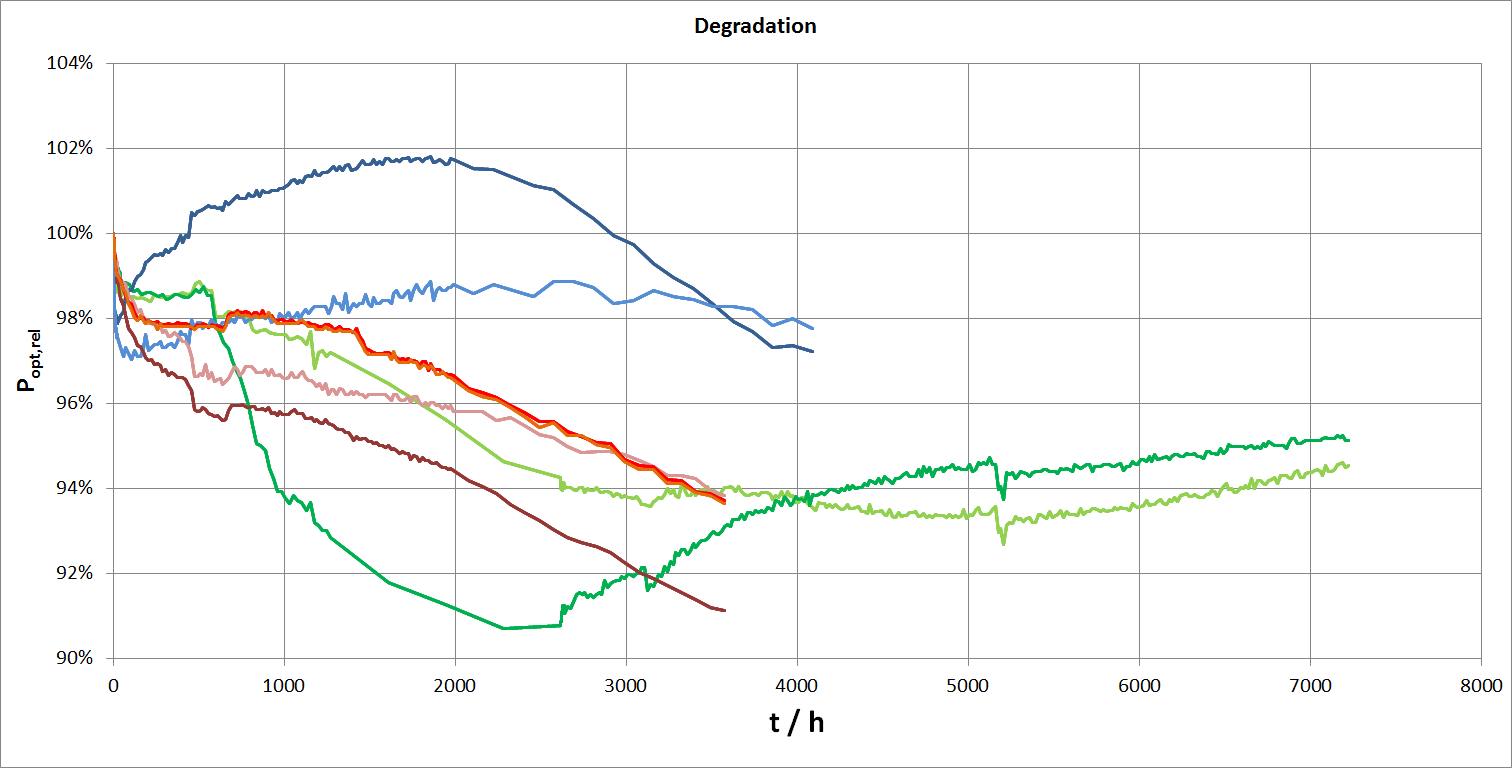
\includegraphics[width=0.8\textwidth]{img/general/Degradation.png}
\caption{Beispiel Degradation}
\label{figure_Degradation}
\end{center}
\end{figure}



\section{Qt}
\label{section_Qt}
Qt ist eine umfangreiche C++-Klassenbibliothek zur Gestaltung und Entwicklung von Anwendungen. Vor allem bei Applikationen mit grafischen Benutzeroberflächen (englisch: \ac{GUI}) ist Qt sehr beliebt. \\
Zusätzlich bringt Qt eine große Auswahl an Tools und Modulen mit sich, welche die Programmierung erheblich erleichtern (z.B. Netzwerkprogrammierung, Datenbankanbindung, OpenGL, etc.). \\
Ein weiterer Vorteil ist die Plattformunabhängigkeit. So unterstützt Qt aktuell (Version 5.4, 10. Dezember 2014) einen Großteil der aktuellen Betriebssystem wie Windows, Linux, Android, iOS und einige mehr. Diese wird dadurch gegeben, dass Qt die meisten Systemaufrufe abstrahiert.

\subsection{Signale und Slots}
\label{QtSignaleSlots}
Die Kommunikation unter den Objekten in Qt erfolgt über Signale und Slots. Dabei sendet ein Objekt ein Signal aus und ein anderes empfängt dieses. Dafür muss zunächst eine Verbindung zwischen den Objekten aufgebaut werden. Das erfolgt mit dem \textit{connect}-Statement.\\

\begin{lstlisting}[caption={Qt \textit{connect}-Statement},label=lst_QtConnect]
connect(Calculate, SIGNAL(clicked()), this, SLOT(addAB()));
\end{lstlisting}

Im Quellcode \ref{lst_QtConnect} wird ein Beispiel für die Verbindung von zwei Objekten mit dem \textit{connect}-Statement gezeigt. Hier wird das Signal \textit{clicked()} des Objektes \textit{Calculate} mit dem Slot \textit{addAB()} des Objektes \textit{this}, was dem aktuellen Objekt entspricht, verbunden. \\

\begin{lstlisting}[caption={Qt \textit{emit}-Statement},label=lst_QtEmit]
void Calculate::my_function(){
	/*
	Do Something
	*/
	emit clicked();	
}
\end{lstlisting}

Im Quellcode \ref{lst_QtEmit} wird das Signal \textit{clicked()} mittels \textit{emit}-Statement ausgelöst und der Slot des verbundenen Objekts aktiviert. Somit ist es möglich beispielsweise die GUI und den Hauptprogrammablauf von einander zu trennen und lediglich über Signale und Slots kommunizieren zu lassen. Dadurch agieren beide Teile komplett unabhängig von einander.

\subsection{Entwicklungsumgebung}
Als Entwicklungsumgebung (englisch: \ac{IDE}) dient der Qt Creator (siehe Abbildung \ref{QtCreator}), welcher Teil des \ac{SDK} von Qt ist und sowohl auf Linux, Windows als auch Mac OS X zur Verfügung steht. Er kommt mit einem Debugger, einem integrierten grafischen \ac{GUI} Designer und einem Texteditor mit Funktionen wie Syntax-Hervorhebung und automatischer Vervollständigung. \\
Dabei kommen gängigen Compiler wie MinGW unter Windows zum Einsatz und es besteht die Möglichkeit eigene Toolchains anzulegen. \\

\begin{figure}[h]
\begin{center}
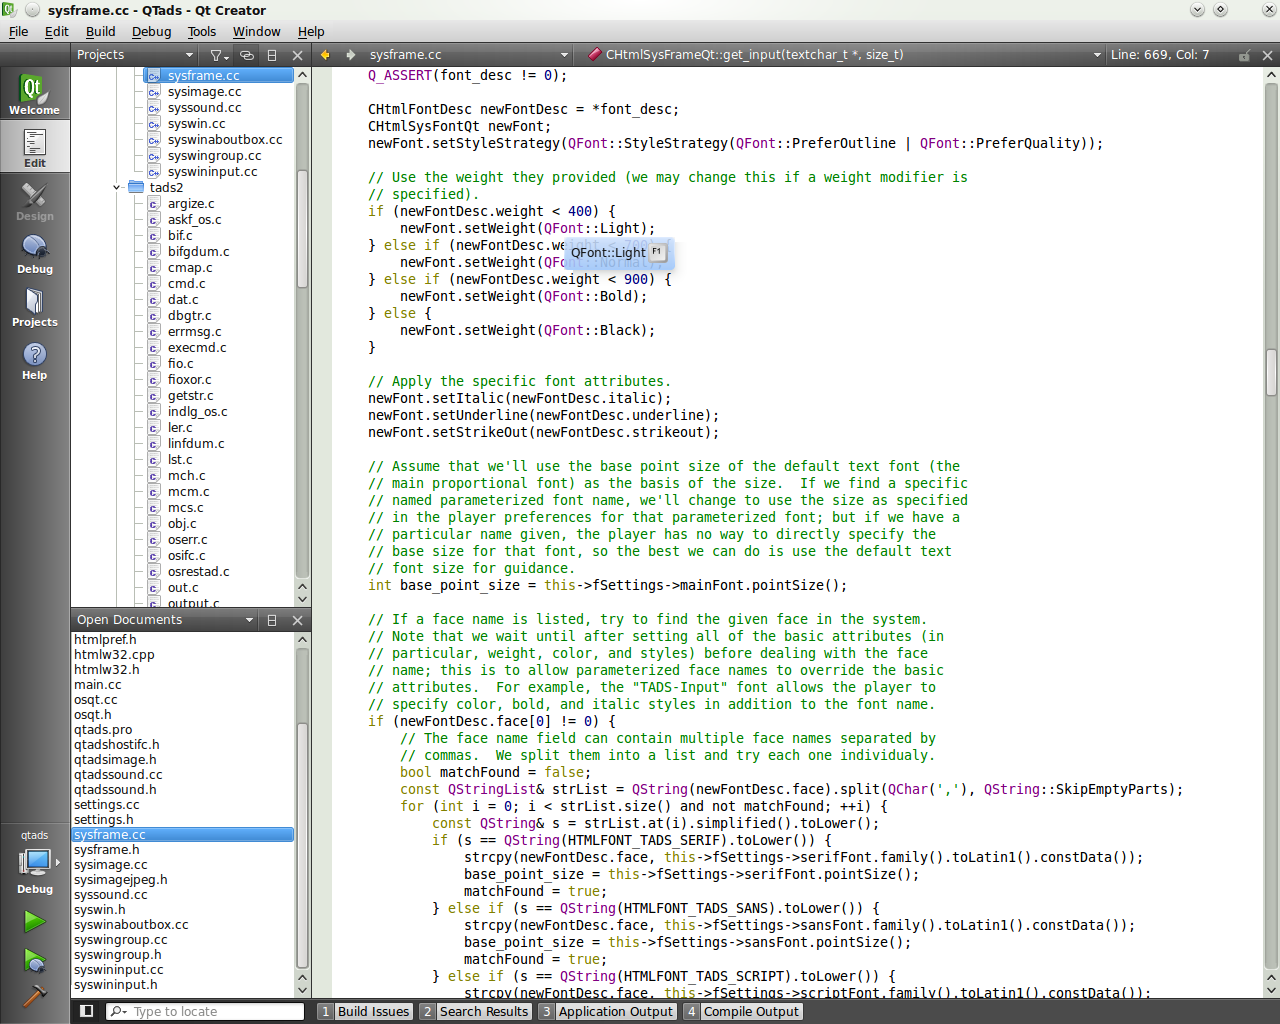
\includegraphics[width=0.8\textwidth]{img/general/QtCreator.png}
\caption{QtCreator Version 2.0.1}
\label{QtCreator}
\end{center}
\end{figure}
\newpage
%Quellen:\\
%http://de.wikipedia.org/wiki/Qt_%28Bibliothek%29
%http://www.mathematik.uni-ulm.de/sai/ws02/cpp/070103/Qt.pdf
%http://wiki.ubuntuusers.de/Qt
%http://en.wikipedia.org/wiki/Qt_Creator


\section{Datenbank}
\label{section_Datenbank}

Für das Speichern der Messdaten und Betriebsparameter wird eine \ac{SQL} \ac{DB} verwendet. Bei der Wahl des \ac{DBMS}, standen mehrere Optionen zur Auswahl und die Entscheidung wurde zwischen SQLite und MySQL gefällt.
Beide System haben ihre Vor- und Nachteile.


\textbf{SQLite} ist ein \ac{SQL} \ac{DBMS}, welches ohne einen Server auskommt und operiert stattdessen in einer einzigen Datei. Es wird vor allem im Embedded Bereich eingesetzt, da kaum Konfigurationen oder Verwaltung notwendig ist. Deshalb eignet es sich ausgezeichnet für sich schnell weiterentwickelnde Applikationen.
\\
Aufgrund dieser Eigenschaften existieren allerdings auch Nachteile. So unterstützt SQLite nur eingeschränkt mehrere Nutzer gleichzeitig. Da das gesamte \ac{DBS} in einer einzigen Datei zusammengefasst ist, können mehrere zur selben Zeit durchgeführte Schreibzugriffe nicht unterstützt werden. Denn die einzige Sicherstellung der Datenintegrität erfolgt durch das Betriebssystem. 
\\
Des Weiteren ist SQLite aufgrund des Ein-Datei-Systems nur eingeschränkt skalierbar. Bei einer größeren Datenmenge oder erhöhten Anzahl an Zugriffen ist es nicht möglich diese Datei auf mehrere Systeme zu separieren, um somit die Last gleichmäßig zu verteilen.

\textbf{MySQL} ist ein weiteres \ac{SQL} \ac{DBMS}, welches allerdings auf einer Serverarchitektur beruht. 
Es ermöglicht die Verwaltung von Nutzern und Rechte. Außerdem ist das System gut hinsichtlich Performance und Größe zu skalieren. Zusätzlich bietet MySQL viele Möglichkeiten für Performanceanpassungen, wie z.B. Query-Caching.
\\
Jedoch gibt es auch hier Nachteile. So ist die Konfiguration wesentlich schwerer und komplexer. Durch die Notwendigkeit eines Servers benötigt MySQL mehr Ressourcen auf dem Host-System.

Die Wahl fällt auf das relationale \ac{DBMS} MySQL. Auch wenn SQLite einige Vorteile vor allem im Embedded Bereich besitzt, ist die fehlende Unterstützen von mehreren Nutzern gleichzeitig ein Ausschlusskriterium.

\cite{saake2010datenbanken}

\newpage

\section{Embedded Linux System}
\label{section_EmbeddedLinux}

Ein eingebettetes System (englisch: \textbf{embedded system}) ist laut \cite{bender2005embedded} ein Rechner, der in ein Gerät oder ein Maschine eingebettet ist und von außen nicht als solcher zu erkennen, sondern lediglich als Träger intelligenter Systemfunktionen sichtbar ist. Des Weiteren übernehme es dabei Überwachungs-, Steuerungs- oder Regelaufgaben.\\
Eingebettete Systeme sind oft spezifisch für die gegebene Aufgabe konzipiert. Dadurch ist es möglich die Hard- und Softwarekonfiguration des Systems zur Verminderung der Kosten und Maximierung der Leistung zu optimieren. Zu finden sind sie in den unterschiedlichsten Bereichen, beispielsweise in mobilen Geräten, industriellen Maschinen, Netzwerkhardware und Verbrauchergeräten.\ 

Ein Embedded Linux (deutsch: eingebettetes Linux) ist ein Betriebssystem, das auf dem Linux-Kernel basiert und in einem eingebetteten System zum Einsatz kommt. \cite{yaghmour2008building} sagt, dass Embedded Linux dabei typischerweise für ein Komplettsystem, bzw. ein Betriebssystem für ein spezifisches eingebettetes Gerät steht. Außerdem verwende man dabei den normalen Linux-Kernel, der sich lediglich in betriebsbedingten Eigenschaften des Zielsystems unterscheide.\ 

Das Embedded Linux System setzt sich aus einem Linux-Kernel nutzenden Rechner, dem Embedded Linux Betriebssystem mit für den Zielrechner passender Software und Werkzeugen für die Entwicklung zusammen. Diese Werkzeuge sind eine Entwicklungsumgebung mit Debugger und Cross-Compiler.

Vorteil ist die Abstraktion der Hardware. Über die Schnittstelle des Kernels kann mit einfachen Systemaufrufen mit der Hardware kommuniziert werden ohne die genaue Hardware komplett zu verstehen.
